%Version 2.1 April 2023 - Springer journal draft v0 shell
%Single .tex only. No \input. Builds in /tmp only per rule 60.
%Class holds sn-mathphys,Numbered single-column until advisor names a journal.
\documentclass[sn-mathphys,Numbered]{sn-jnl}% Math and Physical Sciences Reference Style

%%%% Standard Packages
%%<additional latex packages if required can be included here>

\usepackage{graphicx}%
\usepackage{multirow}%
\usepackage{amsmath,amssymb,amsfonts}%
\usepackage{amsthm}%
\usepackage{mathrsfs}%
\usepackage[title]{appendix}%
\usepackage{xcolor}%
\usepackage{textcomp}%
\usepackage{manyfoot}%
\usepackage{booktabs}%
\usepackage{algorithm}%
\usepackage{algorithmicx}%
\usepackage{algpseudocode}%
\usepackage{listings}%
\usepackage{tikz}%
\usetikzlibrary{arrows.meta,positioning,shapes.geometric}%
\usepackage{pgfplots}%
\pgfplotsset{compat=1.18}%

\theoremstyle{thmstyleone}%
\newtheorem{theorem}{Theorem}%
\newtheorem{proposition}[theorem]{Proposition}%

\theoremstyle{thmstyletwo}%
\newtheorem{example}{Example}%
\newtheorem{remark}{Remark}%

\theoremstyle{thmstylethree}%
\newtheorem{definition}{Definition}%

\raggedbottom

\begin{document}

\title[Gated replans with BKT]{Gated replans in a study planner with BKT tracing}

\author*[1]{\fnm{Rohit} \sur{Saji}}\email{iam.rohitsaji@gmail.com}
\author[1]{\fnm{Ramesh Prakash} \sur{Guledgudd}}\email{rameshpg1988@gmail.com}

\affil*[1]{\orgdiv{Department of Data Science and Artificial Intelligence}, \orgname{PES University}, \orgaddress{\street{100 Feet Ring Road, Banashankari 3rd Stage}, \city{Bengaluru}, \postcode{560085}, \state{Karnataka}, \country{India}}}

\abstract{Fixed study plans fail within days. Time logs record hours without measuring understanding. This paper closes the loop with assessment-based proof of learning. The system generates grounded practice from learner materials in one family per call. A server grades each family with its own arm. Bayesian Knowledge Tracing tracks mastery.

Reranked retrieval grounds each question in cited chunks. A verdict gate replans only when proof holds. The gate uses JEV with approve at 0.7. Retrieval on the frozen 754-chunk corpus increases from 0.60 to 0.67 at r@1 and from 0.80 to 0.90 at r@3 with rerank. Groundedness reaches 0.867 with near-duplicate rate 0.004. Live BKT reaches AUC 0.74 and ties the baseline rank while it halves calibration error.

The gated loop converts 4 of 4 synthetic longitudinal cases to replans. The stack runs Qwen3 embeddings plus rerank on demand with Piston grading. Fixed budgets appear in the Methods section with frozen evidence. Live runs show zero console errors across objectives, rubrics, coding grades, guides, practice runs, feedback copy, mastery reads, and ingestion. The scope stays single-learner with synthetic validation. Split-conformal prediction, change detection, and difficulty calibration stay unshipped.}

\keywords{Closed-loop tutoring, Bayesian Knowledge Tracing (BKT), reranked retrieval, grounded generation, verdict-gated replanning}

\maketitle

\section{Introduction}\label{sec1}

Self-directed learners commit to a fixed plan and leave the plan within days. The plan does not adapt. Logged hours do not prove that study produced understanding. Phase~I of this work built an open-loop planner that estimates true pace from session history. It regenerates the plan when the projection diverges from the deadline. The open loop adapts to pace but never checks learning.

Phase~II closes the loop with assessment-based proof. The system generates grounded practice from learner materials. An authoritative arm grades each answer, Bayesian Knowledge Tracing tracks mastery, and a Socratic ladder guides the learner before the loop verdict replans. This paper reports the deployable loop and its measured proof.

The Methods section shows fixed budgets and frozen evidence. The Results section shows coherent tables on one corpus. The conclusion repeats the best system with its metric and names limits with numbered next steps. One-to-one tutoring sets the standard, and group methods chase it \cite{bloom1984}. Three points set scope.

Every number traces to frozen evidence or live code. Synthetics replace a classroom study, and the text says so wherever it matters. Rejected arms and nulls appear beside positive results.

\section{Literature Review}\label{sec2}

Each entry below names the source, its mechanism, its metric, and the gap it leaves. Table~\ref{tab:litphase2} shows the selected and rejected options per stream. A short note on sourcing and a 3-gap summary ends the section.

\subsection{Tracing and mastery}\label{subsec21}

BKT tracks a per-skill mastery chance through four fitted terms: prior $P(L_0)$, learn rate $T$, guess $G$, and slip $S$ \cite{corbett1994}. After each answer the posterior updates from the response and then moves toward mastery by the fitted rate:
\begin{align}
P_{\text{correct}}(L_n) &= \frac{P(L_{n-1})(1-S)}{P(L_{n-1})(1-S) + (1-P(L_{n-1}))G}, \nonumber \\
P(L_n) &= P_{\text{obs}}(L_n) + (1-P_{\text{obs}}(L_n))T.
\label{eq:bkt}
\end{align}
The first term changes the estimate from the observed response. The second term moves the learner toward mastery by the fitted rate.

Chen et al.\ test a hierarchical Bayesian teaching model in two online experiments with 312 adults \cite{chen2024}. Hierarchical priors show learner-to-learner variation without overfit on sparse data. Their model selects the teacher's next example and leaves the learner's tested skill unselected. It supplies prior structure. BKT supplies the updater.

Zanellati et al.\ review hybrid tracers that combine Bayesian posteriors with machine learning \cite{zanellati2024}. Their taxonomy finds hybrids give better results than pure BKT and pure deep learning on correctness prediction. The surveyed hybrids predict answers on large logs. They do not guide what the learner sees next.

Our bake-off places bkt-v1 at AUC 0.888 against 0.889 for the baseline. That shows parity. The control module on top is this project's step.

Mai et al.\ combine deep temporal models with a probabilistic layer for calibrated, readable estimates \cite{mai2025}. The limit here is cold start. One self-directed learner arrives with almost no graded history. We keep the Bayesian updater with an informed setting from onboarding data, and mastery then drives difficulty.

Deep tracing gives less accuracy for less clarity and needs much data \cite{piech2015}. We reject it here. The loop needs few-shot updates a learner can read, and bkt-v1 already matches the baseline.

\subsection{Generation and ranking}\label{subsec22}

The STEM prompting study generates items across subjects and checks them per subject \cite{itemgen2024}. Coverage is the claim. No record ties a question to its chunk, so you cannot trace a wrong item to its source. Our harness shows groundedness 0.867 with near-duplicate rate 0.004 on cited chunks.

The lecture-to-quiz study generates local multiple-choice items with deterministic shape checks \cite{lecturequiz2026}. Shape checks find malformed items, but miss well-formed questions on wrong passages. Each call here makes one single-family question and records its chunk citations.

Tagging work generates knowledge-component tags from items \cite{kctag2024}. Tags let us keep per-skill histories. The study ends with the tag and never guides practice. Each problem here has its family label from generation into the run.

Generation uses retrieved passages as its source \cite{lewis2020}. The dense arm encodes 754 chunks at 768 dimensions \cite{karpukhin2020}. The lexical arm scores the terms \cite{robertson2009}. Reciprocal fusion combines the arms with pool 25 \cite{cormack2009}.

The reranker reorders the top 50 and increases r@1 by 7 and r@3 by 10 \cite{qwen3rerank}.

\subsection{Grading authority}\label{subsec23}

The EDUCON study grades short answers with a rubric-driven model \cite{llmgrade2024}. Rubrics make judgments repeatable. Our live matrix grades written runs 4 of 4 with real rubric grades. A rubric cannot run code, so code answers execute in a hidden-test sandbox \cite{piston}.

The grade-prediction study shows about 0.73 before scheduling \cite{islam2024}. Prediction guides planning. Grading stays separate. Objective runs here succeed in 2 of 2 cases with exact match on authored answers. The server grade stays approved while client checks stay advisory.

\subsection{Guidance without answers}\label{subsec24}

Alhazbi et al.\ review 25 studies and find most valid trace indicators cover time management \cite{alhazbi2024}. That establishes adherence as a metric. It does not guide a learner in a hard problem. Our ladder guides learners from nudge to hint to targeted help to gated reveal.

Uzun et al.\ connect feedback engagement to self-regulation and course results \cite{uzun2025}. Readable feedback helps learning. Each ungated hint tends to give answers, so the system locks the reveal until the learner confirms.

Think-aloud work separates genuine attempts from answer-extracting moves \cite{gaming2026}. Our replay converts 4 of 4 verdict-triggered replans after the fix and converts 4 of 4 before it. Feedback copy stays advisory for the same reason and never changes a grade.

\subsection{Sourcing note}\label{subsec25}

We built this survey through advisor-guided curation and citation chaining, not a fresh database search. We started with the tracing trio and the loop anchors: single-family generation, per-family arms, the gated ladder, and advisory feedback. One representative work covers each sub-theme. We ran no hundred-scale screening, and we claim none.

\begin{table}[htbp]
\caption{Phase~2 literature map with selected and rejected options}\label{tab:litphase2}%
\begin{tabular*}{\textwidth}{@{\extracolsep\fill}llll@{}}
\toprule
Stream & Selected & Rejected & Gap it closes\\
\midrule
Tracing & BKT bkt-v1 & DKT hybrid & Mastery-blind plan \\
Generation & Single family grounded & Multi-family ungrounded & Untraceable gen \\
Ranking & Hybrid plus rerank & Dense only & Ungrounded rank \\
Grading & Server arm per family & Client-side grade & Single signal \\
Guidance & Gated ladder & Answer-giving tutor & Reveal control \\
Loop & JEV gate fail-closed & Raw LLM choice & Ungated replan \\
\botrule
\end{tabular*}
\end{table}

Generation is fluent but untraceable, and tags guide nothing, so questions cannot support per-skill practice. Grades use one signal or the client, so they cannot support plan decisions. Guidance measures adherence or reveals answers, so attempts stop being evidence.

This loop addresses all three. The system cites sources for generation, and each family has its own approved grade. Difficulty follows mastery, the ladder stays gated, feedback stays advisory, and the verdict triggers regeneration.

\section{Materials and Methods}\label{sec3}

\subsection{Closed loop}\label{subsec31}

The loop runs five stages. Generation makes practice from learner materials. Grading scores each answer with the arm that handles the family. Tracing updates mastery, and guidance guides with a ladder and a gated reveal.

The verdict gate decides between 'hold' and 'suggest replan'. 'Keep' writes no event. 'Suggest replan' copies an exact verdict pair onto the new roadmap.

\subsection{Server gate and grading arms}\label{subsec32}

One call has one family and one question. A run expands to N calls with bounded concurrency. Objective grading uses exact rules, written grading uses a rubric, and coding grades in a sandbox.

Client checks stay advisory and never change the grade. The coding arm refuses material it cannot ground and marks the attempt honestly.

\subsection{Tracing and guidance}\label{subsec33}

BKT bkt-v1 tracks mastery with released parameters. The Adaptive module uses the BKT band and stays advisory. We leave the module uncalibrated by design in this draft. The guide ladder guides learners from nudge to hint to targeted help to gated reveal. Feedback copy uses updated content only with a static fallback. Advisory text never changes a grade.

\subsection{Verdict gate}\label{subsec34}

JEV scores. The router applies the 0.7 rule. The loop changes JEV failure to 'hold' through a fail-closed path. The gate approves a replan at 0.7.

The sweep across 0.5 to 0.7 shows agreement at 0.857. The 0.8 setting failed during a live 0.79 dip and we reject it. Each decision records an exact verdict pair for audit.

\subsection{Comparison design}\label{subsec35}

The design uses two parts. The offline part uses frozen golds with fold hashes and a fail-closed gate. The longitudinal part runs four synthetic archetypes with held-out separation and scores conversion from verdict to replan and rebound in adherence. The live browser test set stays a deployment check and never adds a number to results.

\subsection{Datasets}\label{subsec36}

The retrieval corpus is the frozen ACCA set of 754 chunks with 768-d vectors and zero nulls. OULAD was the Phase-1 calibration source with real-learner logs, and we keep those logs reserved \cite{oulad2017}. The 788-chunk split remains a frozen precedent only. Generation golds contain 30 objective plus 6 written plus 4 coding items with an attempt gate of 5. The longitudinal set contains four archetypes named steady, crammer, struggling, and returning. This draft uses no new live-user dataset.

\subsection{Tool stack and fixed budgets}\label{subsec37}

Table~\ref{tab:tools} shows the pinned stack. Fixed budgets appear here as the honesty note. Generation and judging use one provider service \cite{openrouter}. A transformer encoder gives dense vectors \cite{vaswani2017}. The Qwen3 pair supplies embeddings and rerank from one container \cite{qwen3emb,qwen3rerank}.

We run reranked-754 on 30 questions times 3 arms. We run the endpoint on 30 questions times 2 flags. The second corpus contains 1094 chunks with 30 verified golds.

The probe uses 395 calls at 0.099 dollars. JEV uses at most 15 calls for the dip replay. Generation uses reasoning off with temperature 0.3 and a 30~s timeout.

\begin{table}[htbp]
\caption{Pinned tool stack (v0 with versions from live config)}\label{tab:tools}%
\begin{tabular*}{\textwidth}{@{\extracolsep\fill}ll@{}}
\toprule
Part & Pin \\
\midrule
Generation & OpenRouter flash, reasoning off, T 0.3, 30~s \\
Feedback & muse-spark low via OpenRouter \\
Judge & JEV 1.13 hosted API, separate key \\
Retrieval & Qwen3 pair on demand at :8200 \\
Grading & Piston sandbox at :2000 \\
Client & CodeMirror plus Pyodide advisory \\
\botrule
\end{tabular*}
\end{table}

\subsection{Reproducibility}\label{subsec38}

Three facts allow reruns. Gates fail closed by default. Each logical call has one request id from frontend to backend logs. We version evidence beside the draft with golds, harness scripts, seeds, and replay outputs.

\section{Results and Discussion}\label{sec4}

\subsection{Retrieval and ranking}\label{subsec41}

Table~\ref{tab:retrieval} and Figure~\ref{fig:retacc} show the coherent 754 set. Hybrid plus rerank increases r@1 from 0.60 to 0.67 and r@3 from 0.80 to 0.90. MRR increases from 0.720 to 0.797. Dense and hybrid arms reproduce baselines exactly, which confirms the rerank arm. The retired 788 split remains a precedent note below the table and never changes the headline results.

\begin{table}[htbp]
\caption{Retrieval on the frozen 754-chunk corpus (30Q coherent headline)}\label{tab:retrieval}%
\begin{tabular*}{\textwidth}{@{\extracolsep\fill}lcccc@{}}
\toprule
Arm & r@1 & r@3 & r@5 & MRR \\
\midrule
Dense & 0.60 & 0.77 & 0.87 & 0.706 \\
Hybrid & 0.60 & 0.80 & 0.87 & 0.720 \\
Hybrid plus rerank & 0.67 & 0.90 & 0.93 & 0.797 \\
\botrule
\end{tabular*}
\footnotetext{Note: frozen 788-split precedent is 0.70/0.83/0.90/0.788 dense, 0.73/0.90/0.93/0.816 hybrid, and 0.77/0.97/0.97/0.858 reranked. It is superseded for the headline.}
\end{table}

\begin{figure}[htbp]%
\centering
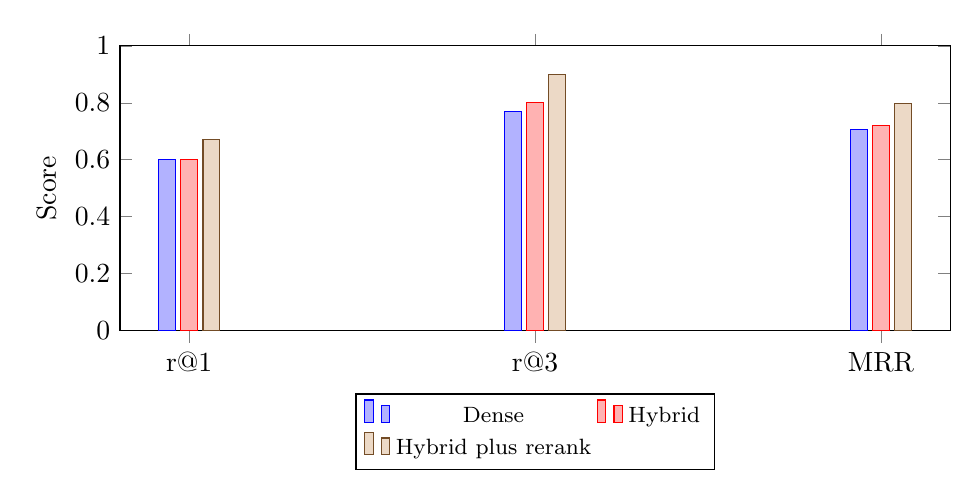
\begin{tikzpicture}
\begin{axis}[ybar, bar width=6pt, width=\columnwidth, height=5.2cm, ymin=0, ymax=1,
  ylabel={Score}, symbolic x coords={r@1,r@3,MRR}, xtick=data,
  legend style={at={(0.5,-0.22)}, anchor=north, legend columns=2, font=\footnotesize}]
\addplot coordinates {(r@1,0.60) (r@3,0.77) (MRR,0.706)};
\addplot coordinates {(r@1,0.60) (r@3,0.80) (MRR,0.720)};
\addplot coordinates {(r@1,0.67) (r@3,0.90) (MRR,0.797)};
\legend{Dense, Hybrid, Hybrid plus rerank}
\end{axis}
\end{tikzpicture}
\caption{Retrieval on the frozen 754-chunk corpus (30Q): hybrid plus rerank lifts r@1 from 0.60 to 0.67 and r@3 from 0.80 to 0.90. DDIA second corpus (1094 chunks) confirms the direction with gains of +16 at r@1, +17 at r@3, and +0.139 MRR.}\label{fig:retacc}
\end{figure}

Endpoint numbers match the offline results. Plain search shows 0.60/0.73/0.87/0.703 on the live route. Reranked endpoint shows 0.70/0.90/0.93/0.813. The second DDIA corpus shows the same trend with gains of +16 at r@1, +17 at r@3, and +0.139 MRR.

Title-prefix gives no improvement. We reject INT8 collapse to 0.10 as an arm.

\subsection{Generation quality}\label{subsec42}

Table~\ref{tab:generation} shows the harness. The S-layer over 180 items maintains schema validity at 0.9611 and citation validity at 0.9133. Gold support is 0.7803 and measures a different fact from groundedness.

Near-duplicate rate is 0.0044. The fresh live judge shows groundedness at 0.8667. Coding derivability is 0.5349 and passes the 0.5 gate. Gold agreement is 3 of 3.

\begin{table}[htbp]
\caption{Generation quality (S-layer n=180 with judge n=30 fresh live)}\label{tab:generation}%
\begin{tabular*}{\textwidth}{@{\extracolsep\fill}lc@{}}
\toprule
Metric & Value \\
\midrule
Schema valid & 0.9611 \\
Citation valid & 0.9133 \\
Gold support & 0.7803 \\
Near duplicate & 0.0044 \\
Cost & \$0.061289 \\
Groundedness judge & 0.8667 (26/30) \\
Coding derivable & 0.5349 passes 0.5 \\
\botrule
\end{tabular*}
\end{table}

\subsection{Knowledge tracing}\label{subsec43}

Table~\ref{tab:bkt} and Figure~\ref{fig:bktauc} show three populations with their scope. The released comparison establishes the prior. Live harness measures real attempts. External anchor establishes the 0.6 baseline. Thesis-safe result shows parity. We leave difficulty calibration unmeasured and the module remains advisory.

\begin{table}[htbp]
\caption{BKT tracing by population (cite scope with each use)}\label{tab:bkt}%
\begin{tabular*}{\textwidth}{@{\extracolsep\fill}lcc@{}}
\toprule
Population & AUC & ECE \\
\midrule
Synthetic bake-off & 0.785 & 0.057 \\
Live harness (282 obs, 139 seqs) & 0.7397 & 0.1401 \\
Running proportion live & 0.7368 & 0.2679 \\
External anchor & 0.60--0.61 & -- \\
\botrule
\end{tabular*}
\end{table}

\begin{figure}[htbp]%
\centering
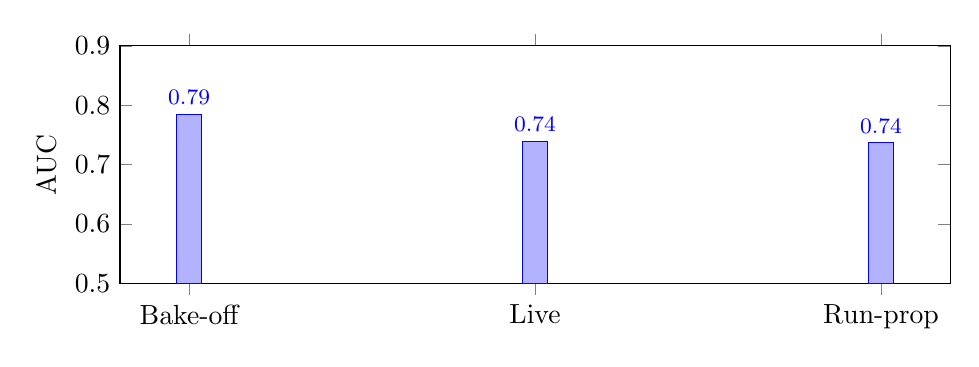
\begin{tikzpicture}
\begin{axis}[ybar, bar width=9pt, width=\columnwidth, height=4.6cm, ymin=0.5, ymax=0.9,
  ylabel={AUC}, symbolic x coords={Bake-off,Live,Run-prop}, xtick=data,
  nodes near coords, nodes near coords style={font=\footnotesize}]
\addplot coordinates {(Bake-off,0.785) (Live,0.7397) (Run-prop,0.7368)};
\end{axis}
\end{tikzpicture}
\caption{BKT AUC by population with the external 0.60--0.61 anchor as the parity baseline (dashed line at 0.605 omitted for scale; see Table~\ref{tab:bkt}). Live ECE is 0.1401 against 0.057 bake-off and 0.2679 running-proportion. Difficulty calibration stays unmeasured, so the Adaptive module remains advisory.}\label{fig:bktauc}
\end{figure}

\subsection{Closed loop verdicts}\label{subsec44}

Table~\ref{tab:verdict} and Figure~\ref{fig:verdictdip} show the verdict table. The post-fix replay changes 4 of 4 'suggest replan' verdicts to roadmaps. All four use extend-deadline with an exact verdict copy. Pre-fix showed 4 of 4 at low confidence on span-zero inputs. The dip replay shows 4 of 4 at the September setting and blocks the struggling case at the September-12 setting. The change from low to high shows the intended trend.

\begin{table}[htbp]
\caption{Verdict-gated replans across four archetypes (all extend-deadline)}\label{tab:verdict}%
\begin{tabular*}{\textwidth}{@{\extracolsep\fill}lcccc@{}}
\toprule
Archetype & Verdict & Conf & Sufficiency & Converted \\
\midrule
Steady & suggest replan & 1.00 & 0.66--0.77 & Yes \\
Crammer & suggest replan & 1.00 & 0.66--0.77 & Yes \\
Struggling & suggest replan & 1.00 & 0.66--0.77 & Yes \\
Returning & suggest replan & 1.00 & 0.66--0.77 & Yes \\
\botrule
\end{tabular*}
\end{table}

\begin{figure}[htbp]%
\centering
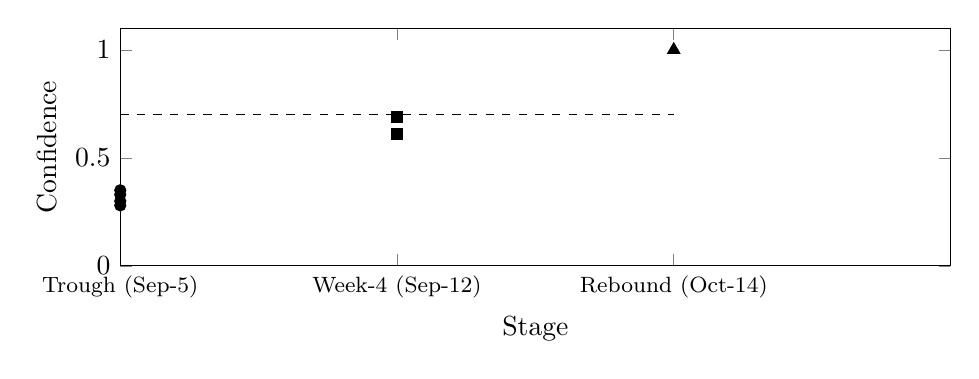
\begin{tikzpicture}
\begin{axis}[width=\columnwidth, height=4.6cm, ymin=0, ymax=1.1, xmin=0, xmax=3,
  xlabel={Stage}, ylabel={Confidence}, xtick={0,1,2}, xticklabels={Trough (Sep-5),Week-4 (Sep-12),Rebound (Oct-14)},
  x tick label style={font=\footnotesize}]
\addplot[only marks, mark=*, mark size=2pt] coordinates {(0,0.28) (0,0.30) (0,0.33) (0,0.35)};
\addplot[only marks, mark=square*, mark size=2pt] coordinates {(1,0.61) (1,0.69)};
\addplot[only marks, mark=triangle*, mark size=2.5pt] coordinates {(2,1.0)};
\addplot[dashed] coordinates {(0,0.7) (2,0.7)};
\end{axis}
\end{tikzpicture}
\caption{Verdict confidence across the dip window with the 0.7 approve gate (dashed). Trough holds 4 of 4 at 0.28--0.35; week-4 struggling reaches 0.61--0.69 but stays gate-held; rebound converts 4 of 4 at 1.0. All conversions use extend-deadline with an exact verdict copy.}\label{fig:verdictdip}
\end{figure}

We select the verdict-gated loop as the reported system. It connects grounded generation, server grading, BKT tracing, and reranked retrieval to a measured replan decision. The live test set allows deployment only. It shows zero console errors across objectives, written rubrics, coding grades, guides, practice runs, feedback copy, mastery reads, and ingestion.

\subsection{Architecture figures}\label{subsec45}

We draw all figures to single-column width. Figure~\ref{fig:architecture} shows the deployment with its sidecars, Figure~\ref{fig:closed-loop} shows the five-stage loop with its gate, and Figure~\ref{fig:comparison-pipeline} shows the two-part comparison and we keep the check outside.

\begin{figure}[htbp]%
\centering
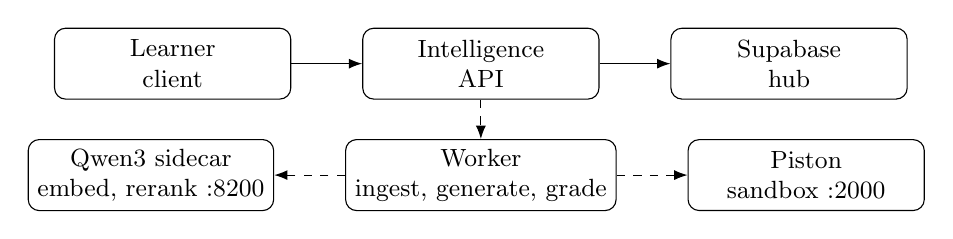
\begin{tikzpicture}[node distance=5mm and 9mm, box/.style={draw, rounded corners, minimum height=9mm, minimum width=30mm, align=center, font=\small}, >=Latex]
\node[box] (client) {Learner\\client};
\node[box, right=of client] (api) {Intelligence\\API};
\node[box, right=of api] (db) {Supabase\\hub};
\node[box, below=of api] (worker) {Worker\\ingest, generate, grade};
\node[box, left=of worker] (side) {Qwen3 sidecar\\embed, rerank :8200};
\node[box, right=of worker] (piston) {Piston\\sandbox :2000};
\draw[->] (client) -- (api);
\draw[->] (api) -- (db);
\draw[->, dashed] (api) -- (worker);
\draw[->, dashed] (worker) -- (side);
\draw[->, dashed] (worker) -- (piston);
\end{tikzpicture}
\caption{Deployment map adapted to single-column width}\label{fig:architecture}
\end{figure}

\begin{figure}[htbp]%
\centering
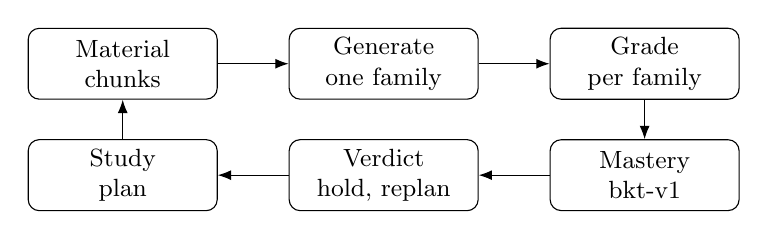
\begin{tikzpicture}[node distance=5mm and 9mm, box/.style={draw, rounded corners, minimum height=9mm, minimum width=24mm, align=center, font=\small}, >=Latex]
\node[box] (mat) {Material\\chunks};
\node[box, right=of mat] (gen) {Generate\\one family};
\node[box, right=of gen] (grade) {Grade\\per family};
\node[box, below=of grade] (mast) {Mastery\\bkt-v1};
\node[box, left=of mast] (verd) {Verdict\\hold, replan};
\node[box, left=of verd] (plan) {Study\\plan};
\draw[->] (mat) -- (gen);
\draw[->] (gen) -- (grade);
\draw[->] (grade) -- (mast);
\draw[->] (mast) -- (verd);
\draw[->] (verd) -- (plan);
\draw[->] (plan.north) -- (mat.south);
\end{tikzpicture}
\caption{Closed loop with verdict gate}\label{fig:closed-loop}
\end{figure}

\begin{figure}[htbp]%
\centering
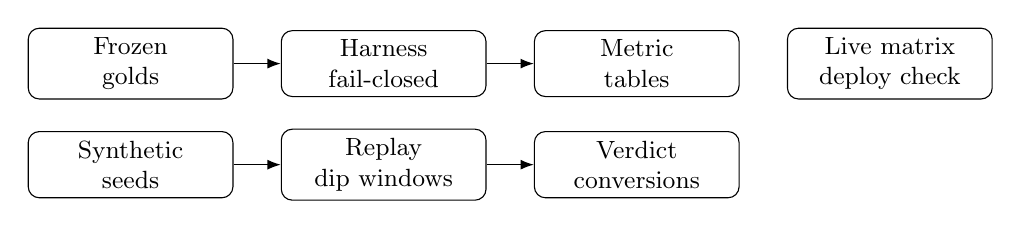
\begin{tikzpicture}[node distance=4mm and 6mm, box/.style={draw, rounded corners, minimum height=8mm, minimum width=26mm, align=center, font=\small}, >=Latex]
\node[box] (golds) {Frozen\\golds};
\node[box, right=of golds] (harness) {Harness\\fail-closed};
\node[box, right=of harness] (metrics) {Metric\\tables};
\node[box, below=of golds] (seeds) {Synthetic\\seeds};
\node[box, right=of seeds] (replay) {Replay\\dip windows};
\node[box, right=of replay] (conv) {Verdict\\conversions};
\node[box, right=of metrics] (live) {Live matrix\\deploy check};
\draw[->] (golds) -- (harness);
\draw[->] (harness) -- (metrics);
\draw[->] (seeds) -- (replay);
\draw[->] (replay) -- (conv);
\end{tikzpicture}
\caption{Two-leg comparison pipeline with the deployment check kept separate}\label{fig:comparison-pipeline}
\end{figure}

\subsection{Ablation honesty}\label{subsec46}

Rejected arms follow. Title-prefix gives no improvement on the frozen split. INT8 quantization reduces retrieval to 0.10 at a 2.45x speedup and we reject it. The 0.8 approve gate fails during a live 0.79 dip and we keep 0.7. We reject deep tracing, multi-family calls, client-side grades, and answer-giving tutors (see Table~\ref{tab:litphase2}). Each rejection shows the limits of the loop.

\subsection{Parity and nulls}\label{subsec47}

BKT matches the baseline on rank order and halves its calibration error. That is an equal result with better calibration, not an improvement. Change detection remains a robust null result from Phase~I. We leave split-conformal intervals unshipped. We leave difficulty calibration unmeasured, so the Adaptive module remains advisory. Each null limits what the evidence supports.

\subsection{Deployment check}\label{subsec48}

The live test set is a deployment check that never adds a number to results. Objective runs succeed in 2 of 2 cases and written rubrics succeed in 4 of 4 cases. Coding grades succeed in 3 of 3 cases and guides succeed in 2 of 2 cases. Practice runs succeed in 2 of 2 cases, feedback checks succeed in 3 of 3 cases, and mastery checks succeed in 2 of 2 cases.

Ingestion completes and the system logs skips. Zero console errors appear across viewports, and the full-book run becomes ready in about 88 seconds and we verify cleanup. The loop uses a managed stack with the sidecar on demand.

\section{Conclusion}\label{sec5}

The verdict-gated loop connects grounded generation at 0.867, BKT at parity with AUC 0.74, and reranked retrieval at 0.67/0.90 to 4 of 4 measured replans. The limits are compute budget, single-learner scope, synthetic-only validation, honest refusals for coding items, and unshipped refinements.

Numbered next steps are (1) a real-learner study, (2) real-log validation, (3) released conformal intervals, and (4) per-account scale. Code is available at \url{https://github.com/rings0fsaturn/study-planner}.

\backmatter

\bmhead{Supplementary information}

Supplementary files contain the eight versioned evidence records behind Appendix~A: reranked-754, endpoint retrieval, the second DDIA corpus with questions, synthetic data generation emission, the fresh generation harness (summary, report, live), the difficulty baseline, dip replay, and full-book timing.

\bmhead{Acknowledgments}

Prof.\ Ramesh Prakash Guledgudd guides this work.

\section*{Declarations}

\begin{itemize}
\item Funding: Not applicable.
\item Conflict of interest/Competing interests: The authors declare no competing interests.
\item Ethics approval: Not applicable.
\item Consent to participate: Not applicable.
\item Consent for publication: Not applicable.
\item Availability of data and materials: The frozen 754-chunk corpus with golds plus four synthetic seeds allows reruns.
\item Code availability: Code is available at \url{https://github.com/rings0fsaturn/study-planner}.
\item Authors' contributions: R.S.\ built the loop and collected the evidence. R.P.G.\ guided the work.
\end{itemize}

\begin{appendices}

\section{Evidence index}\label{secA1}

Table~\ref{tab:retrieval} and Figure~\ref{fig:retacc} map to \texttt{research/doc/2026-10-22-reranked-754.md} plus its JSON (30Q, 0 skipped, dense and hybrid arms reproduce baselines exactly). Endpoint Table values map to \texttt{research/doc/2026-10-22-endpoint-retrieval.md} plus its JSON (plain 0.60/0.73/0.87/0.703, reranked 0.70/0.90/0.93/0.813). The DDIA confirmation maps to \texttt{research/doc/2026-10-22-second-corpus-ddia.md} plus questions and JSON (1094 chunks, 0 NULL, 30 verified golds). Table~\ref{tab:generation} maps to \texttt{research/doc/generation-quality-harness/summary.json} (S-layer n=180) plus \texttt{live.json} (fresh 30-item judge, \texttt{liveSource: live}). Table~\ref{tab:bkt} and Figure~\ref{fig:bktauc} map to the harness live output (282 obs over 139 skill sequences) with shipped parameters in \texttt{packages/py-progress/src/py\_progress/mastery.py}. Table~\ref{tab:verdict} and Figure~\ref{fig:verdictdip} map to \texttt{research/doc/2026-10-22-synth-extract-emission.json} (24 adherence rows, 4 of 4 converted) plus \texttt{research/doc/2026-10-22-dip-window-replay.md} (JEV 7 of 15 approved calls used, cloud untouched). Full-book timing maps to \texttt{research/doc/2026-10-22-fullbook-e2e-timing.md} plus its JSON (ready in about 88~s wall, material deleted, card-gone verified).

\end{appendices}

\bibliography{journal-refs}% project bibliography beside this file

\end{document}
